\section{Week 8}

\subsection{Completions}
For a ring $R$, the completion of $R$ w/r/t a maximal ideal $\mathfrak m \subset R$ is the inverse limit
\[
    \tilde{R} = \left( \frac{R}{\mathfrak m} \leftarrow \frac{R}{\mathfrak m^2} \leftarrow \frac{R}{\mathfrak m^3} \cdots \right).
\]
That is, elements of $\tilde{R}$ are sequences $a_1 \leftarrow a_2 \leftarrow \dots$ such that
\[
    a_i \in \frac{R}{\mathfrak m^i}, \quad a_{i+1} \mapsto a_i \text{ via the natural map } \frac{R}{\mathfrak m^{i+1}} \to \frac{R}{\mathfrak m^i}.
\]
The standard example of completions is the completion of $k[x]$ w/r/t to $(x)$. Then
\[
    \tilde{k[x]} = \left( \frac{k[x]}{(x)} \leftarrow \frac{k[x]}{(x^2)} \leftarrow \frac{k[x]}{(x^3)} \cdots \right).
\]
Elements of $\tilde{k[x]}$ are of the form $c_1 \leftarrow c_1 + c_2x \leftarrow \dots$ so $\tilde{k[x]} = k[[x]]$, the space of formal power series.

In general, we may ask if the natural map $R \to \tilde{R}$ is injective (i.e. if we lose information via completion). We will show that if $R$ is a local Noetherian ring, then completion w/r/t to the unique maximal ideal will result in an injective embedding. To do this, we need two often-used lemmas: Nakayama's and Artin-Rees.

\paragraph{Nakayama's Lemma.} Nakayama's lemma states if $M$ is a f.g. module over a local ring $R$ with maximal ideal $\mathfrak m$, then $\mathfrak m M = M \implies M = 0$. The proof is pick a finite set of generators $a_1, \dots, a_n$ of $M = \mathfrak m M$, and observe we can write.
\[
    a_1 = \sum a_i m_i, \quad m_i \in \mathfrak m
\]
As $\mathfrak m$ is the unique maximal ideal of $R$, thus $1 - m_1$ is invertible, and we can write $a_1$ as a linear combination of $a_i$, $i > 1$. Doing this repeatedly, we can reduce the number of generators to 0.

\paragraph{Artin-Rees Lemma.} Define a decreasing filtration of module $M$ to be a chain
\[
    M = M_0 \supset M_1 \supset M_2 \supset \dots.
\]
Call such a filtration stable if there exists ideal $I$ such that
\[
    M_{i+1} \supset IM_{i}
\]
with equality for large $i$. The most common example of filtrations is the chain
\[
    M \supset IM \supset I^2M \supset \dots
\]
called the $I$-adic filtration. Filtrations also give rise to a (translation invariant) topology on $M$ by defining a basis of neighborhoods around 0 to be the sets $M_i$. Note that any two stable filtrations give rise to the same topology. (Filtrations also play a role in many important constructions, like blow-up algebras or turning noncommmutative rings into commmutative ones.)

The Artin-Rees lemma states for f.g. modules $M \subset N$ over Noetherian ring $R$, any stable filtration (with ideal $I$) of $N$ restricts to a stable filtration over $M$. The key observation of the proof is to note:
\[
    \begin{split}
        & M_i \text{ is a stable filtration }\\
        & \iff M_0 \oplus M_1 \oplus \dots \text{ is a graded module f.g. over the graded ring}\\
        & \quad \quad \quad R \oplus I \oplus I^2 \oplus \dots.
    \end{split}
\]
A-R then follows with noting that b/c $R$ is Noetherian, $N_0 \oplus N_1 \oplus \dots$ being f.g. implies that $M_0 \oplus M_1 \oplus \dots$ is f.g.

To show that a local Noetherian ring $R$ can be embedded into its completion $\tilde{R}$, we do the following:
\begin{enumerate}
    \item Let $J = \bigcap \mathfrak m^n$. To show $J = 0$, we first apply A-R to the filtration
    \[
        R \supset \mathfrak mR \supset \mathfrak m^2R \supset \dots
    \]
    to show that restricted to $J$, we have the stable filtration
    \[
        J = J \cap \mathfrak m = J \cap \mathfrak m^2 = \dots
    \]
    which gives rise to the indiscrete topology. 
    \item We thus conclude that all stable filtrations on $J$ give rise to the indiscrete topology. In particular, this means
    \[
        J \supset \mathfrak mJ \supset \mathfrak m^2J \supset \dots
    \]
    gives rise to the indiscrete topology, so $J = \mathfrak m J$, which implies $J = 0$ by Nakayama.
\end{enumerate}

\subsection{Survey of Module Properties}
Here is an overview of various module properties related to finiteness.
\begin{figure}[H]
    \centering
    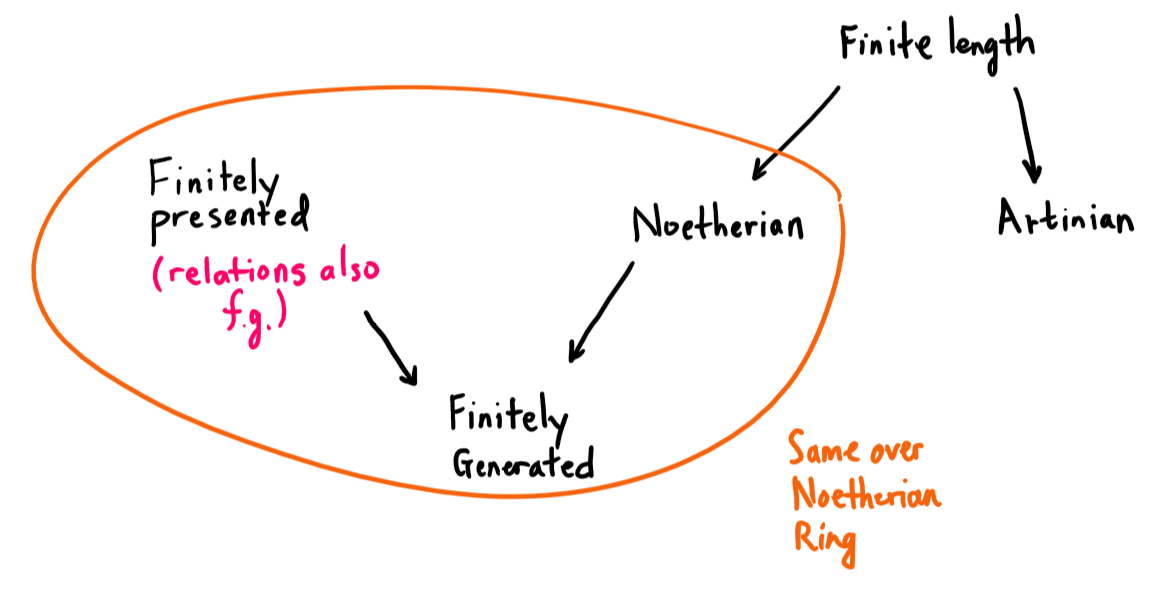
\includegraphics[width=\linewidth]{figures/finiteness.png}
\end{figure}

Here is an overview of various module properties related to freeness.
\begin{figure}[H]
    \centering
    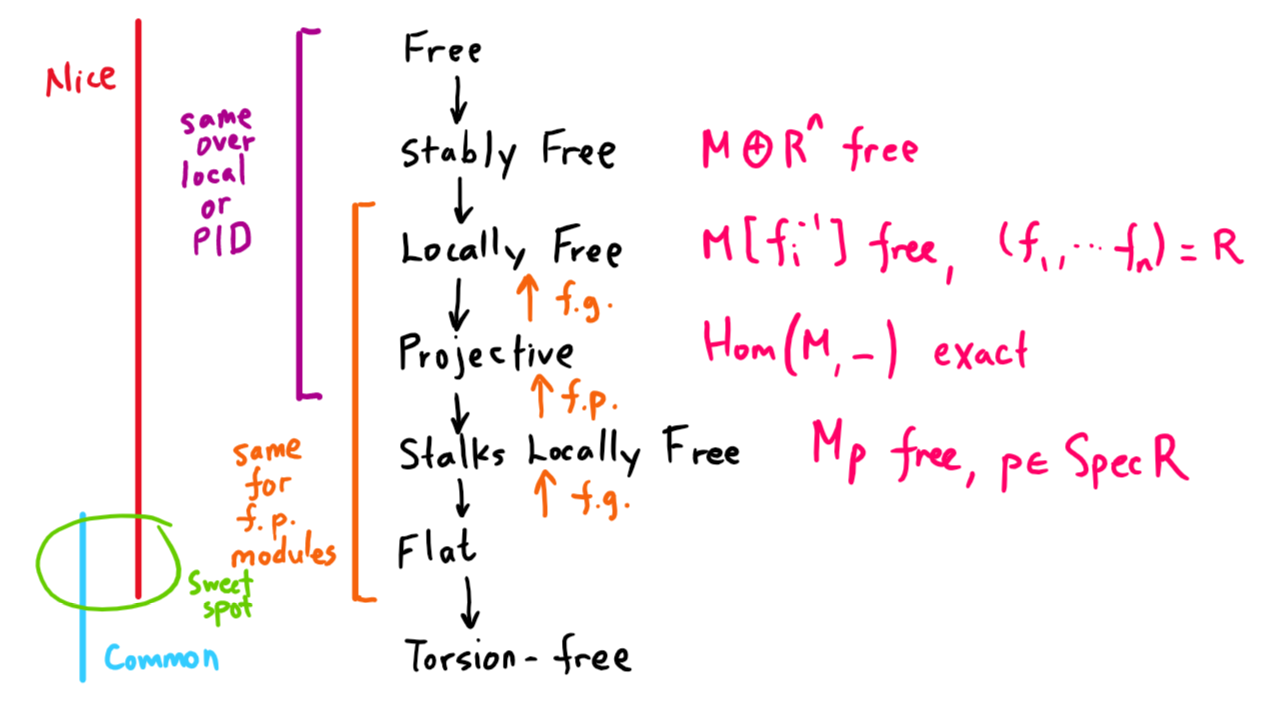
\includegraphics[width=\linewidth]{figures/module-cheat-sheet.png}
\end{figure}

\subsection{Stably Free Modules}
Call a $R$-module $M$ stably free if $M \oplus R^n$ is free for some $n < \i$.

An example of a stably free module that is not free comes from topology. Let $R$ be the ring of continuous functions on $S^2$ and $M$ the module of continuous vector fields on $S^2$ ($R$ acts on $M$ via pointwise multiplication). Let $TS^2$ denote the tangent bundle of $S^2$ (i.e. the disjoint union of $T_xS^2$ over all $x \in S^2$) and $NS^2$ denote the normal bundle of $S^2$ (similar definition). Then note
\[
    M: S^2 \to TS^2, \quad R: S^2 \to NS^2
\]
so
\[
    M \oplus R: S^2 \to TS^2 \oplus NS^2
\]
thus
\[
    M \oplus R: S^2 \to \bR^3 \implies M \oplus R \cong R^3.
\]
So $M$ is stably free. However $M$ is not free, a fact that can be deduced from the Hairy Ball theorem, which states that any continuous vector field over $S^2$ must have a vanishing point.

In general, because many algebraic invariants behave the same way over both free and stably free modules, it is often hard to distinguish between the two.

\subsection{The Mazur Swindle Trick}
The swindle trick works as follows: suppose we are given objects $A, B$ such that $A + B = 0$ (whatever that means). If we can define infinite sums of these objects that behave well, then we can conclude $A = B = 0$.

The argument is to note
\[
    0 = (A + B) + (A + B) + \dots = A + (B + A) + (B + A) + \dots = A.
\]
Although a simple trick, the swindle can be used to proved nontrivial statements. For instance, one can show that joining together two nontrivial knots cannot produce a trivial knot. That is, knots cannot ``undo'' each other.

Applying the swindle trick to modules where we define $M + N = 0$ if $M \oplus N = $ free, we can prove that projective modules (i.e. summands of free module) are precisely the modules $M$ such that $M \oplus R^n$ is free for some (possibly infinite) $n$. And if we do some clever manipulation, we can also show that all stably free modules of infinite rank (i.e. $M \oplus R^n = R^\i$) are free.

\subsection{Locally Free Modules}
Tangent and normal bundles over a manifold are special cases of vector bundles. A vector bundle assigns each point on a manifold a vector space such that there is nice and compatible behavior. More formally, a vector bundle over a manifold $X$ is a nice map
\[
    f: V \to X
\]
such that the fibers (i.e. preimages of points) are vector spaces and such that locally $f$ looks like the projection 
\[
    \bR^n \times U \to U.
\]
A section is a map that (nicely) assigns each point on the manifold a element in the corresponding vector space (e.g. for tangent bundles, sections are continuous vector fields). In other words, a right inverse of $f$.

Call a $R$-module $M$ locally free if the modules $M[f_i^{-1}]$ over some finite open cover $R[f_i^{-1}]$ of $R$ are free (open cover in the sense of the spectrums). Given a vector bundle, the module of sections over the ring of continuous functions on the manifold is a typical example of a locally free module. This is because due to the local behavior of $f$, the space of sections defined over local $U$ is $\bR^n$.

\subsection{Projective Modules}
In commutative algebra (i.e. over commutative rings), locally free modules are projective. However, in general, depending on what objects you study, locally free things may or may not be projective, a fact that has led to a lot of confusion in the literature. 

\subsection{Flat and Torsion-Free Modules}
Flat modules are arguably the most important class of modules because they are relatively common (unlike projective/free/locally free modules) and generally nice. Torsion-free modules are more common, but not as nice, so we don't really study them.

%%% Local Variables:
%%% TeX-master: "main"
%%% End: